\documentclass[12pt]{article}

\usepackage{graphicx}
\usepackage{url}
\usepackage{amsmath}
\usepackage[cm]{fullpage}
\usepackage{calc}
\usepackage{subfig}
\usepackage{float}

\title{\textbf{Wireless and Mobile Computing, Assignment 6}}
\author{Marcel Mohler \& Thomas Richner}
\begin{document}
\maketitle

\section{Setup}

We use a scenario where one station is a receiver and two stations send traffic to this receiver. Both sending stations make use of two ACs, hence send two data flows to the receiving station. The receiver therefore has four incoming flows.
We put all stations at the coordinates (0,0).

\begin{figure}[h!]
\centering
\includegraphics[width=80mm]{img/setup.png}
\caption{setup, receiver station and two sending stations \label{fig:setup}}
\end{figure}


\section{Algorithm Design "Anna"}

\subsection{Design Goals}
Our goal is to maximize the throughput per station under the following two constraints in order of their priority:
\begin{enumerate}
  \item Complete fairness against stations using the same algorithm which also results in no starvation. In case of two stations, both should achieve 50\% of the maximal throughput.
  We do not care about stations not using our algorithm at all.
  \item Basic 802.11e QoS support. We always prioritize AC1 over AC2. But if AC1 does not use the channel completely, AC2 should be allowed to fill it up.
\end{enumerate}

\subsection{Implementation}
We use a shared-counter based arbitration method to slice the available channel capacity into time slots. Each station aquires its own time slot and only contends for the channel during the allocated slot. But once it is contending, it uses very aggressive parameters. Hence there is no backoff and the \texttt{CW\_min} and \texttt{AIFSN} are set to the minimum.
In order to emulate the non-contending behaviour during other stations time slots we use  \texttt{CW\_min} and \texttt{AIFSN} parameters in the order of 1000. As long as we have no unknown opponents we can keep the collisions approximately at zero since there is no real contention between multiple stations.

Since our goal is to maximise relative and not necessarily absolute throughput, we do not  modify phymode or power parameters.

\subsection{Pseudo-Code}

\includegraphics[width=160mm]{img/pseudocode.png}



\section{Evaluation}
In the following measurements we modeled a primitive opponent as a simple algorithm that randomly increases or decreases its AC01 AIFSN. 
\subsection{Random vs. Random}
We display the throughout over time of two Random Algorithms competing over the channel.
Since both stations are using a very simple algorithm the expected throughput is relativly low. The measurement confirms this hypothesis. Both algorithms average around 1 Mb/s throughput. The dotted, red line shows the total channel capacity of 5 Mb/s and we are clearly way below that theoretical maximum.

\begin{figure}[h!]
\centering
\includegraphics[width=\textwidth]{img/random_vs_random-50Mbps-PLOT.png}
\caption{MAC parameters over time of our random algorithm \label{plot:rr}}
\end{figure}

\begin{figure}[h!]
\centering
\includegraphics[width=\textwidth]{img/random_vs_random.png}
\caption{throughput per station and time, two random algorithms \label{fig:rr}}
\end{figure}

\subsection{Anna vs. Anna}
In this measurement we tried the performance of two Anna algorithms as station 02 and station 03.
As mentioned in the design section, this is where our algorithm should perform a fair TDMA, which means that both stations send by turns without the interference of the other one.
This is visible in Figure 4 where station 2 (blue) and station 3 (green) achieve a throughput of almost the channel capacity.
Figure 5 provides a screenshot of Jemula which shows that there are indeed close to zero collisions due to the nature of TDMA.
\begin{figure}[h!]
\centering
\includegraphics[width=\textwidth]{img/anna_vs_anna-5Mbps-TDMA.png}
\caption{throughput per station and time, two Annas. Characteristic TDMA pattern. \label{fig:aa}}
\end{figure}

\begin{figure}[h!]
\centering
\includegraphics[width=\textwidth]{img/Anna_vs_Anna_TDMA.png}
\caption{Channel visualization. Characteristic TDMA pattern. \label{fig:aa}}
\end{figure}

\subsection{Anna vs. Random}
Finally we measured Anna versus the random algorithm described above.
Since Anna does not detect another station using its algorithm it falls into "no-backoff-mode" where it behaves completely selfish and does not care about other stations, resulting in sending all the time with no backoff or AIFS.
Figure 6 plots throughput of both stations against time as well as the channel capacity.
Since the random algorithm uses longer InterFrameSpace and larger contention windows it stays silent for longer periods of time resulting in Anna being able to achieve more throughput.
There are a lot of collisions since Anna sends all the time but in general Anna will have priority.
The measurements show these behaviour and with a channel offer of 5 Mb/s Anna still achieves around 3 Mb/s average throughput while the random algorithm is at around 0.75 Mb/s.
\begin{figure}[h!]
\centering
\includegraphics[width=\textwidth]{img/annaVSrandom_thrp.png}
\caption{throughput per station and time, Anna versus our random algorithm. \label{fig:aa}}
\end{figure}

\begin{figure}[h!]
\centering
\includegraphics[width=\textwidth]{img/annaVSrandom.png}
\caption{Channel characteristics, in favor of STA2.  \label{fig:aa}}
\end{figure}

\subsection{Discussion \& Conclusion}

\subsubsection{Limitations}
In a real world situation our TDMA approach would create relative high synchronization overhead, furthermore it is not as simple to arbitrate the channel in real systems. On the other hand 802.11 already supports RTS/CTS, which can be seen as some kind of dynamic TDMA. RTS/CTS creates a contention free time slot as it is needed, similar to dynamic TDMA. Our agressive MAC parameters are also against the principle of collision avoidance, we even force them against unknown opponents. If the opponent also uses agressive parameters, we may end up in a situation where the channel is busy with collisions and the channel capacity approximates zero.

\section{Feedback}

\begin{description}
  \item[Difficulty] \hfill \\ appropriate
  \item[Clarity] \hfill \\ okay
  \item[Time Spent] \hfill \\ 10h
  \item[Conclusion] \hfill \\ 
\end{description}

\end{document}
